%!TEX TS-program = xelatex
%!TEX root = ../../maxwell2018thesis.tex

\chapter[Searching and Stopping]{Searching and Stopping:\\A Background}
\label{chap:stopping}
Having established the main focus of this thesis, this chapter provides a detailed overview of the current state of the literature in the context of stopping during search, and the varying ways in which it has been examined and subsequently modelled. We examine this from two main perspectives, considering:

\begin{itemize}
    \item{the \textbf{conceptual and descriptive} approaches that have been undertaken; and}
    \item{the \textbf{formalised} approaches that have been examined.}
\end{itemize}

Conceptual and descriptive approaches generally consider a high-level approach of stopping. Approaches taken, as described in this chapter, include a series of \emph{stopping heuristics and rules} (Section~\ref{sec:stopping:heuristics}) and a series of user studies examining the phenomenon and the wider \emph{Information Seeking and Retrieval (ISR)} process~\citep{kelly2013evaluation_review}, as detailed in Section~\ref{sec:stopping:studies}. These approaches generally provide a picture of the domain, with this information subsequently allowing us to develop more formalised approaches~\citep{azzopardi2015theories}.

In turn, formalised approaches are more precise, building upon the knowledge and understanding obtained from the conceptual and descriptive approaches. Generally, a formalised approach enumerates each aspect of the phenomena as a variable, allowing one to explore how varying each variable functionally relates to others. In the context of examining one's stopping behaviour, a number of different formalised ISR models have been proposed, which we discuss in relation to stopping in Section~\ref{sec:stopping:theories}.

\section{User Studies}\label{sec:stopping:studies}
what have studies shown that examine stopping behaviour?

~\cite{wu2014information_scent}\\
~\cite{dostert2009satisficing}\\
~\cite{toms2009predicting_stopping}\\
~\cite{zach2005enough_is_enough}\\
~\cite{wu2014stopping_query_abandonment}\\
~\cite{marchionini1995information_seeking}


\section{Stopping Heuristics}\label{sec:stopping:heuristics}
Despite the inherent difficulties that have been observed when ascertaining how and when people stop searching, researchers have over the years proposed a number of different stopping heuristics which are \emph{believed} to provide a more concrete means of quantifying and/or explaining when searchers decide to stop, and thus quantifying the sense of what is \emph{``good enough''}~\citep{wu2014information_scent}.

A majority of these heuristics can be found within~\gls{ir} research, with the earliest having been defined as far back as the early 1970's. These heuristics are generally high level, \emph{conceptual} approaches that describe when searching should stop, at different levels (e.g. the session level, or the query level). To describe each of the heuristics, we break this section up into a number of different subsections, which provides a loose classification of the different approaches that have been described in the literature. We consider first:

\begin{itemize}
    
    \item{a \emph{fixed-depth} approach, considered as the de facto stopping heuristic used in much~\gls{ir} research today.}
    
\end{itemize}

From this, a series of more \emph{adaptive} heuristics are defined in the literature which we consider in turn. These are:

\begin{itemize}
    \item{tolerance to non-relevance;}
    \item{satiation rules;}
    \item{difference rules;}
    \item{time-based rules; and}
    \item{patch-based rules.}
\end{itemize}

\subsection{The Fixed Depth}
Preciaion-at-k is the classic example here.
You will go to a fixed depth always
Assumed by the cranfield paradigm, for example.

unrealistic. so what other approaches are there in the literature?
a number of different rules are explained in the literature.

\subsection{Cognitive Heuristics}
By far the largest category of stopping heuristics defined within the literature are \emph{cognitive based} heuristics. That is to say, heuristics that attempt to model in some form of criterion or criteria that are met in the mind of the searcher as he or she examines content to determine what is and what is not relevant.

\subsubsection{Tolerance to Non-Relevance}



\citeauthor{cooper1973retrieval_effectiveness} worked on two studies~\citep{cooper1973retrieval_effectiveness, cooper1973retrieval_effectiveness_ii} that argued that the best way in which to evaluate a retrieval system would be to elicit subjective estimates of the system's utility to its users.



It was argued in Part I (see JASIS, March-April 1973 p. 87) that the best way to evaluate a retrieval system is, in principle at least, to elicit subjective estimates of the system's utility to its users, quantified in terms of the numbers of utiles (e.g. dollars) they would have been willing to give up in exchange for the privilege of using the system; and a naive methodology was outlined for evaluating retrieval systems on this basis. But the impracticality of the naive evaluation procedure as it stands raises the questions: How can one decide which practical measure is likely to yield results most closely resembling those of the naive methodology? And how can one tell whether the resemblance is close enough to make applying the measure worth while? In the present paper two kinds of solution to these problems are taken up. The first answers the questions in terms of the reasonableness of the simplifying assumptions needed to get from the naive measure to the proposed substitute. The second answers it by experimentation.


~\cite{cooper1973retrieval_effectiveness}

~\cite{cooper1973retrieval_effectiveness_ii}


cooper.
pretty much the same rule was defined by nickles

considers a searcher's tolerance to non-relevance.


\subsubsection{Satiation Rules}

\subsubsection{Difference}

\subsubsection{The Mental List}

\subsubsection{Representational Stability}

\subsubsection{Magnitude Threshold}

\subsubsection{The Single Criterion}

\subsection{Time-Based}

\subsection{Patch Rules}

\section{Formal Theories of Interaction}\label{sec:stopping:theories}
Understanding the complex behaviours exhibited by searchers during the ISR process has been a longstanding problem~\citep{azzopardi2015theories}. With most approaches considering the direct observation of searcher behaviours through interaction log data as described previously in Section~\ref{sec:stopping:studies}, several attempts have been made to provide mathematically grounded, formalised theories that describe this process. From these theories, one can then begin to deduce a series of testable hypotheses when undertaking interaction studies, such as the hypothesis provided in Chapter~\ref{chap:snippets}, and as published in~\cite{maxwell2017snippets}.

We discuss in this section three main competing ISR theories, all of which provide a rational explanation of \emph{when searchers should stop}.

\begin{itemize}
    \item{\textbf{\emph{Information Foraging Theory (IFT)}}~\citep{pirolli1999ift}, which considers a searcher \emph{foraging} for information to be analogous to an animal foraging for food in the wild -- allowing for the inclusion of many theoretical approaches used in ecology to be applied to search (Section~\ref{sec:stopping:theories:ift});}
    
    \item{the \textbf{\emph{Interactive Probability Ranking Principle (iPRP)}}~\citep{fuhr2008iprp}, allowing for the modelling of a searcher in making decisions, or \emph{choices}, during an interactive search session (Section~\ref{sec:stopping:theories:iprp}); and}
    
    \item{\textbf{\emph{Search Economic Theory (SET)}}~\citep{azzopardi2011economics}, where the search interactions that take place between a searcher and the computer is modelled as an economics problem (Section~\ref{sec:stopping:theories:set}).}
\end{itemize}

Paradoxically, an astute way in which to introduce these formal models is to begin by discussing a \emph{conceptual model} -- the \emph{Berry Picking Model}.

\begin{figure}[t!]
    \centering
    \resizebox{1\hsize}{!}{
    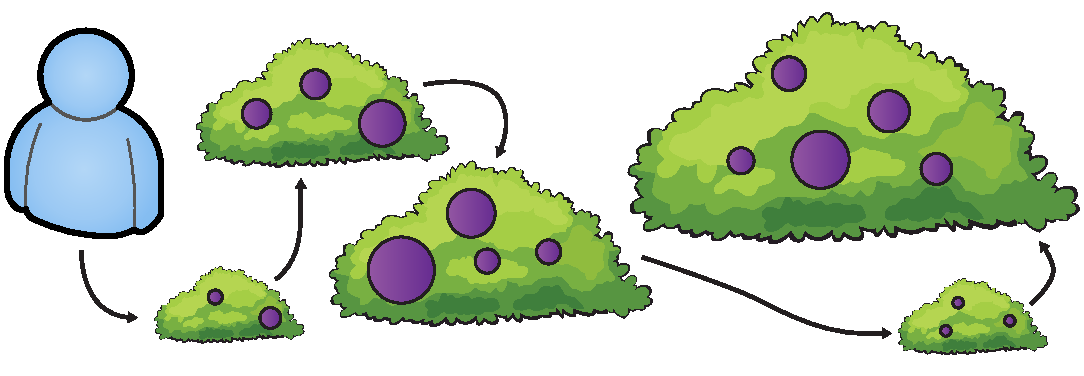
\includegraphics{figures/ch3-berry_picking.pdf}}
    \caption[Berry Picking]{A crude illustration depicting \emph{Bates' Berry Picking model}~\citep{bates1989berry_picking}. In this conceptual model, a berry picker forages through a series of \emph{patches} (refer to Section~\ref{sec:stopping:theories:ift} for more information; patches are represented in the illustration as bushes) in search of the ripest berries (a simple assumption would be to assume larger berries are riper). This model mirrors how an individual searches with an evolving information need.}
    \label{fig:ch3-berry_picking}
\end{figure}

\subsection{From Conceptual to Formal}\label{sec:stopping:theories:conceptual}
As illustrated in Figure~\ref{fig:ch3-berry_picking}, the Berry Picking Model~\citep{bates1989berry_picking} draws an analogy between a searcher and a \emph{forager} -- in this case, a forager looking for berries. The forager attempts to collect the ripest berries within a series of different \emph{patches} (refer to Section~\ref{sec:stopping:theories:ift} for more information on the \emph{patch model}). This is crudely illustrated in Figure~\ref{fig:ch3-berry_picking}, where the forager moves between bushes (patches). Once the ripe berries have been collected from a patch, the forager moves to the next patch, until all patches have been exhausted. The analogy here regarding search considers a patch as a SERP, with a forager here attempting to look for the most relevant documents to their information need. As stated by~\citeauthor{bates1989berry_picking}, the forager's information need evolves, and so the type of information they attempt to find valuable at a given point also changes. Switching back to the berry picking analogy, this may mean a switch between blueberries and strawberries, for example.

While this conceptual model is intuitive and subsequently easy to understand, the model lacks the ability to describe how long a forager will spend in an individual patch, or how long the time taken to reach a patch in the first place will affect their behaviour~\citep{azzopardi2015theories}. The lack of explanation is where more formalised approaches attempt to provide an answer. For example, researchers took forward the concept of a searcher as a forager (e.g.~\cite{russell1993sense_making, sandstrom1994optimal_foraging}), with their results suggesting that \emph{Optimal Foraging Theory (OFT)}~\citep{stephens1986foraging_theory} could be used to model the search process. This subsequently gave rise to the theory of Information Foraging Theory~\citep{pirolli1999ift}.

\subsection{Information Foraging Theory}\label{sec:stopping:theories:ift}
Analogous to an organism foraging for food in the wild, Information Foraging Theory considers a searcher as an \emph{informavore}\footnote{The term \emph{informavore} was originally coined by~\citeauthor{miller1983informavores}. \emph{``Just as the body survives by ingesting negative entropy, so the mind survives by ingesting information. In a very general sense, all higher organisms are informavores.''}}, an organism that consumes \emph{information.} IFT is comprised of a \emph{ternion} of underlying models~\cite{pirolli1999ift}, which are explained below. A graphical illustration of the three models can also be seen in Figure~\ref{fig:ch3-patch}.

\begin{figure}[t!]
    \centering
    \resizebox{1\hsize}{!}{
    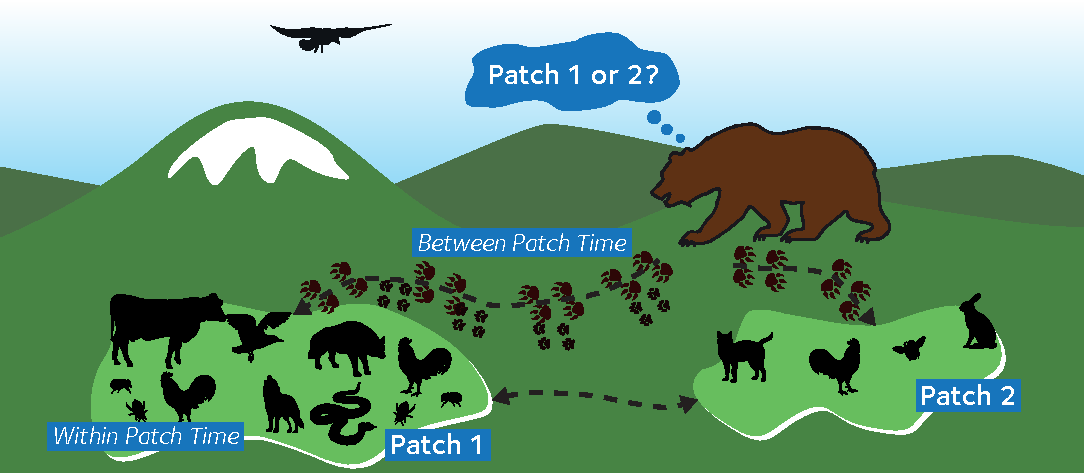
\includegraphics{figures/ch3-patch.pdf}}
    \caption[Illustration of the Patch Model]{A graphical representation of various models that form Information Foraging Theory. Should the forager expend effort navigating to \emph{Patch 1}, or \emph{Patch 2}? \emph{Patch 1} is further away, with a stronger scent, and offers more potential gain (food). However, \emph{Patch 2} is closer. IFT provides a framework for addressing these issues. Also shown within the illustration are the \emph{between patch} and \emph{within patch} times that are spent by the forager. Refer to Section~\ref{sec:stopping:theories:ift} for an explanation on what these times represent. Silhouettes acquired from \emph{freepik.com}.}
    \label{fig:ch3-patch}
\end{figure}

\begin{itemize}
    
    \item{The \textbf{\emph{Information Scent model}} considers how informavores rely upon various \emph{proximal cues}~\citep{chi2001information_scent} (e.g. bolded terms, other textual snippets, or graphics within \emph{information cards} -- see~\cite{bota2016information_cards}, for example) to indicate how promising a particular patch (e.g. a document) looks to be in terms of satisfying their information need. This is analogous to an organism foraging for food; organisms rely upon various cues in the surrounding environment (e.g. paw prints, smells) to guide them to a promising patch. Both informavores and herbivores/carnivores estimate how beneficial following a particular path, or \emph{scent trail}, will be\footnote{A discussion of this explanation can be found by Jakob Nielsen at \url{https://www.nngroup.com/articles/information-scent/} -- last accessed December 7\textsuperscript{th}, 2017.}. Once the scent starts to weaken (i.e. when no more additional information is expected to be found), a informavore will stop and progress to a different scent trail~\citep{piorkowski2012information_scent}.}
    
    \item{The \textbf{\emph{Information Diet model}} -- when considering a webpage as a patch and information as the prey -- provides a rationale for determining which information a forager will consume. Leaving a particular website may be straightforward, but finding a better one is not necessarily so -- although it can be argued that in recent years, the advancement of search engine technology has made this issue to be less of a challenge~\citep{vaughan2004new_measurements}. If it for example is easier for a forager to find lots of potentially useful webpages, there is less incentive for them to stay on a single page; technological developments today encourage the consumption of small chunks of information from a high number of sources, and, as such, a change in our behavioural characteristics.\footnote{The idea of technology changing our behavioural characteristics is not new; an article in the \emph{New York Times} suggests that the development of technology has made us more impatient, expecting instant answers -- and more forgetful, too, in the sense that the relative cost of accessing information is now so low, we readily discard information. The article is available at \url{http://www.nytimes.com/2010/06/07/technology/07brainside.html}, last accessed December 7\textsuperscript{th}, 2017. Refer also to~\cite{carr2008google_stupid}.}}
    
    \item{Finally, \textbf{\emph{Information Patch model}} concerns how long a forager will stay in a particular \emph{patch} (e.g. an area of land, or, in terms of an informavore, a list of ranked documents, for example) before deciding to move to a new patch.}
    
\end{itemize}

We consider the Information Patch model as of particular relevance to the work in this thesis, as it concerns when a forager will \emph{stop} examining a given patch. Given the illustration in Figure~\ref{fig:ch3-ift}, the analogy for an information seeker -- or informavore -- is that:

\begin{itemize}
    \item{\emph{moving between a patch} is like \emph{issuing a new query}, and the subsequent query formulation cost that must be expended; and}
    \item{\emph{staying within a patch} is analogous to \emph{assessing a series of documents}, where each document incurs an examination cost.}
\end{itemize}

With these assumptions in hand, the Information Patch model allows for the prediction of how long a forager should stay in a patch before moving to the next patch. As IFT is based upon Optimal Foraging Theory (OFT)~\citep{stephens1986foraging_theory}, two main assumptions about the forager are made, in that, unsurprisingly, they will act in an optimal fashion:

\begin{itemize}
    \item{the forager will \emph{always enter the patch with the highest potential yield first}; and}
    \item{the forager will \emph{maximise their gain per unit of time} spent in a patch~\citep{pirolli1999ift, stephens1986foraging_theory}.}
\end{itemize}

When considering the sample illustration in Figure~\ref{fig:ch3-patch}, this therefore means that the forager will enter \emph{Patch 1} first, as this patch offers the largest return for the energy the forager initially expends reaching the patch. When considering the stopping behaviour exhibited by a forager, one needs to calculate the gain attained at a given point in time, or $g(t)$. From this, the moment at which a forager should optimally stop examining a patch is the point in time at which the maximal value of gain per unit of time is reached. This is dependent upon a number of factors, including aspects such as the \emph{between patch} and \emph{within patch} times -- the times spent getting to a patch, and spent within a patch, examining content, respectively. 

Figure~\ref{fig:ch3-ift} provides two plots to demonstrate the theory in action, demonstrating on the left a gain. The illustration shows four gain curves that are for individual patches, each under different conditions. We show the difference in stopping times between patches with both a low and high between-patch time (i.e. a longer time to enter the patch from zero time), and patches which are fruitful, giving a high yield, and those with a low yield. By taking the gain curves and drawing the tangent to the curve through the origin, we can then see that the optimal stopping point as dictated by IFT is the point on the gain curve where its tangent intersects with it. This is the point of the \emph{maximal rate of gain}; foragers spending time within the given patch after this point will experience continually diminishing returns. IFT suggests that after this point, a forager should abandon the patch, and then proceed to issue a new query, and subsequently enter a new patch.

\begin{figure}[t!]
    \centering
    \resizebox{1\hsize}{!}{
    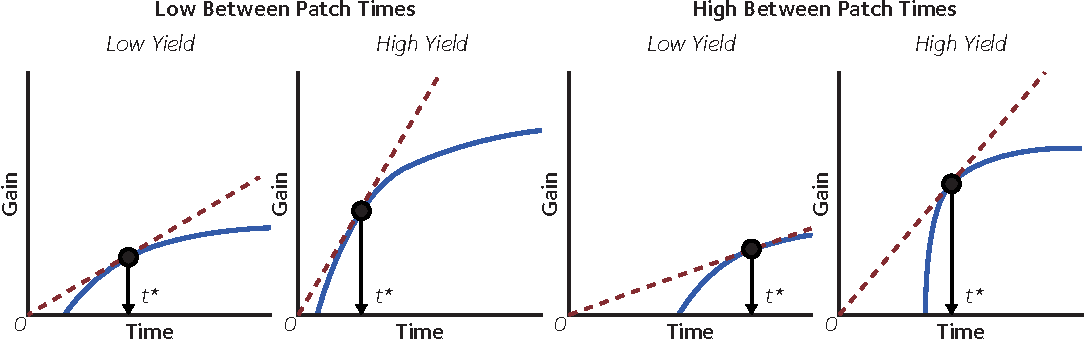
\includegraphics{figures/ch3-ift.pdf}}
    \caption[Plots of optimal patch stopping points for Information Foraging Theory]{Four plots, each denoting a different scenario for the optimal stopping point within a patch, as outlined by \emph{Information Foraging Theory}. The two plots on the left denote a low between-patch time, with the two right plots illustrating a high between patch time. The \emph{Low Yield} plots denote smaller levels of gain per unit of time compared to the \emph{High Yield} patches. Note the optimal stopping point is denoted by \emph{t*}, the point at which the tangent of the gain curve intersects. Time spent within the patch after this point will result in steadily diminishing returns.}
    \label{fig:ch3-ift}
\end{figure}

\vspace{-5mm}
\subsection{Considering Costs and Benefits}
The other means by which information seeking has been formally modelled is through the consideration of the \emph{costs} and \emph{benefits} that a searcher must consider during the search process. Although not discussed in the original Berry Picking model,~\citeauthor{bates1979search_tactics} does discuss the idea that these should be weighed up in subsequent work~\citep{bates1979search_tactics}.

The idea of using a cost/benefit analysis is not new; a number of other formal models have been created using this underlying approach. In~\gls{ir} research for example, purchasing decisions and ranking have been considered using this approach. A more user-centric approach was undertaken by Cooper, who modelled the trade-off between how long a searcher should spend searching, and how much time the system should itself spend searching. More related to the work in this thesis is the \emph{Probability Ranking Principle (PRP)} by~\citeauthor{robertson1977prp}, who proposed a formalised model utilising decision theory to the so-called \emph{ranking problem}~\citep{robertson1977prp}. The PRP essentially formed a theoretical foundation for optimising the results of ad-hoc retrieval. The PRP itself has in past decade been extended to yield the \emph{Interactive Probability Ranking Principle}~\citep{fuhr2008iprp}, as discussed in Section~\ref{sec:stopping:theories:iprp} below.

\subsubsection{The Interactive Probability Ranking Principle}\label{sec:stopping:theories:iprp}
With the PRP considering only the ranking problem, the notion of user interactions during ad-hoc retrieval are largely ignored by this theory. Systems have been shown in previous studies to perform differently in in a standard retrieval setting, of a single query and ad-hoc retrieval (e.g.~\cite{voorhees2000trec8, turpin2006performance_versus_measures}). Using the PRP, this approach is indistinguishable from an interactive setting. Studies have also shown that scanning through a list of ranked documents to identify potentially relevant entries may not be the most crucial activity in the~\gls{iir} process~\citep{turpin2001batch_evaluations}. As such. the iPRP provides and extension to the classical PRP, providing a means of formalising various activities within a search session besides simply scanning a ranked list of results.

Based upon the preexisting PRP, the iPRP removes two key assumptions that the PRP makes to increase the flexibility of the underlying model. These changes include the removal of the assumptions that consider:

\begin{itemize}
    \item{a \emph{fixed information need}, allowing a user modelled by the iPRP to have an information need that changes and adapts as documents are examined (e.g. as per the \emph{Anomalous State of Knowledge (ASK)}, described by~\citeauthor{belkin1980ask}); and}
    \item{the assumption that the \emph{relevance of documents is independent of other documents}.}
\end{itemize}

While sensible assumptions to make for the purposes of modelling, it has been demonstrated that the assumptions do under certain circumstances break down~\citep{gordon1991utility_theory}. From these updated assumptions, three main requirements were specified, namely that iPRP must:

\begin{enumerate}
    \item{consider the interaction process as a whole, rather than simply considering document ranking as was assumed in the classical PRP;}
    \item{allow for different of costs and benefits to be invested and given respectively, meaning that, for example, a longer document will take a greater period of time to examine than a shorter document; and}
    \item{allow for the changing of the information need throughout the course of the search session, \`{a} la~\cite{belkin1980ask}.}
\end{enumerate}

This last point is reminiscent of Bates' Berry Picking model. As outlined in Section~\ref{sec:stopping:theories:conceptual}, a forager would traverse through patches/bushes in order to find the ripest berries available. However, as they forage, they may find, for example, certain berries to be riper than others. As such, they adjust what they are foraging for as they acquire more berries. In terms of an information seeker, this is analogous of a searcher's mental model of a particular topic continually evolving as they are subjected to new information through each document they examine. As such, one's information need may change as new information is uncovered.

From these requirements, the iPRP was then created with four revised assumptions, namely that:

\begin{enumerate}
    \item{there should be a focus on the function level of interaction, meaning that there are a variety of different activities one can undertake (e.g. query formulation, document examination), with each activity having a cost and benefit associated with it;}
    \item{\emph{decisions} forming the basis of interaction;}
    \item{the searcher evaluating the \emph{choices} laid before him/her in a \emph{linear order} (i.e. when examining a list of ranked results, starting from the top and working your way down); and}
    \item{only decisions that are positive and correct are of benefit to the searcher.}
\end{enumerate}

\subsubsection{Search Economic Theory}\label{sec:stopping:theories:set}
The origins of SET can be traced back to work by~\cite{varian1999economics}, who outlined three directions in which 

\section{Chapter Summary}

\begin{itemize}
\item there has been lots of conceptual work on trying to understand stopping behaviours, but most boil down to the fact that people stop because what they have found is “good enough”.
\item despite this, we have all these different heuristics that researchers define — primarilry mental rule that searchers tick off as they go through results. And once a criterion/some criteria have been satisfied, they stop.
\item and now we have theories of information seeking behaviour which also provide us with a mathematical means for trying to deduce when people stop. These are themselves stopping rules.
\item this goes back to what I am saying in chapter 2, which states that most models and measures that we use all encode within them some form of stopping model — they are just not particularly realistic.
\item and from here, we can go: we have these heuristics and rules, but there is nothing in the literature to show how well these rules perform when compared to real behaviours. We know that behaviours change under different search contexts; it therefore follows that stopping behaviour will also change. And so, in order to look at this, we now introduce our conceptual search model (next chapter), before using this model in a series of simulations to ascertain exactly how stopping behaviour changes under different conditions/different search goals (remaining chapters).
\end{itemize}
